\subsection{Positive Ordered Integers Array:}

The first test will consist in evaluate the running time of the algorithms analyzing an array of ordered integers of size $2^{10}$. \hfill \break

\begin{figure}[H]
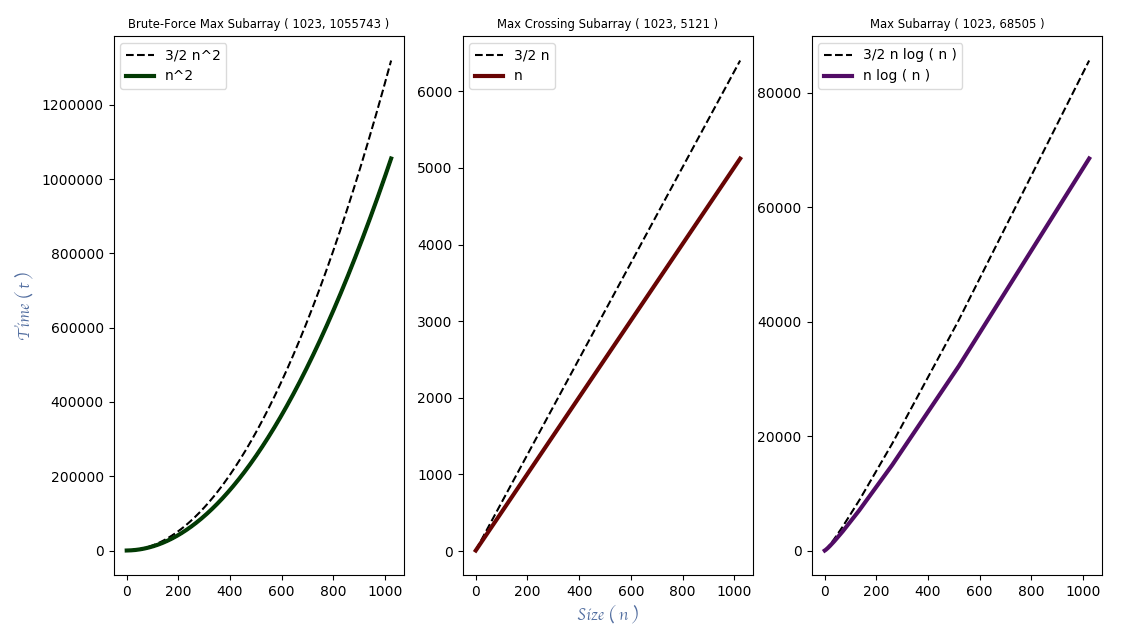
\includegraphics[width = 17cm, height = 10cm]{t1.png}
\centering \linebreak \linebreak Figure 4.1.0: Algorithms results for an array of size $2^{10}$.
\end{figure} \hfill 

{\bfseries\itshape\color{carmine}{Observation:}} {\itshape\color{carmine}{Since the size it's $2^{10}$ the parameters of the points of each algorithm are to many, so we decide to not attach only for this case the table of mapping values and the console output only the plot.}}

\pagebreak

The second test will consist in evaluate the running time of the algorithms analyzing an array of ordered integers of size $2^{5}$. \hfill \break

\begin{figure}[H]
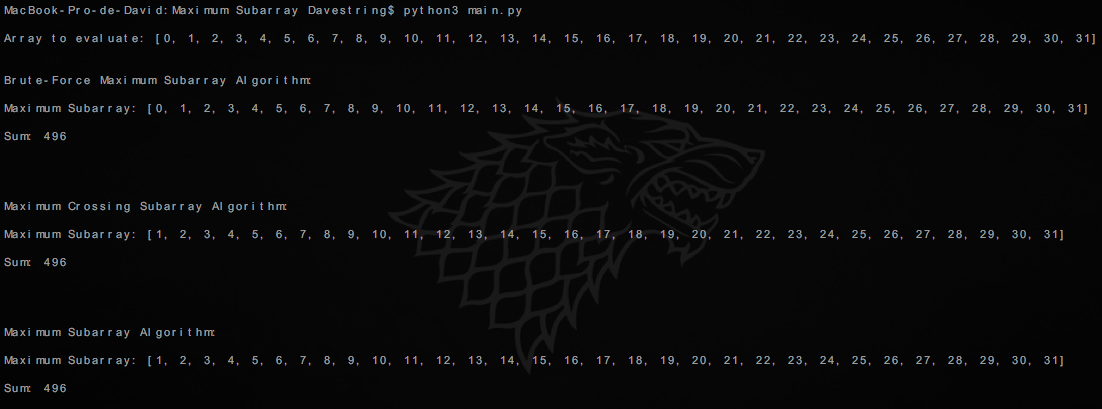
\includegraphics[width = 17cm, height = 10cm]{co2.png}
\centering \linebreak \linebreak Figure 4.1.1: Console output of the program.
\end{figure} \hfill 

\begin{figure}[H]
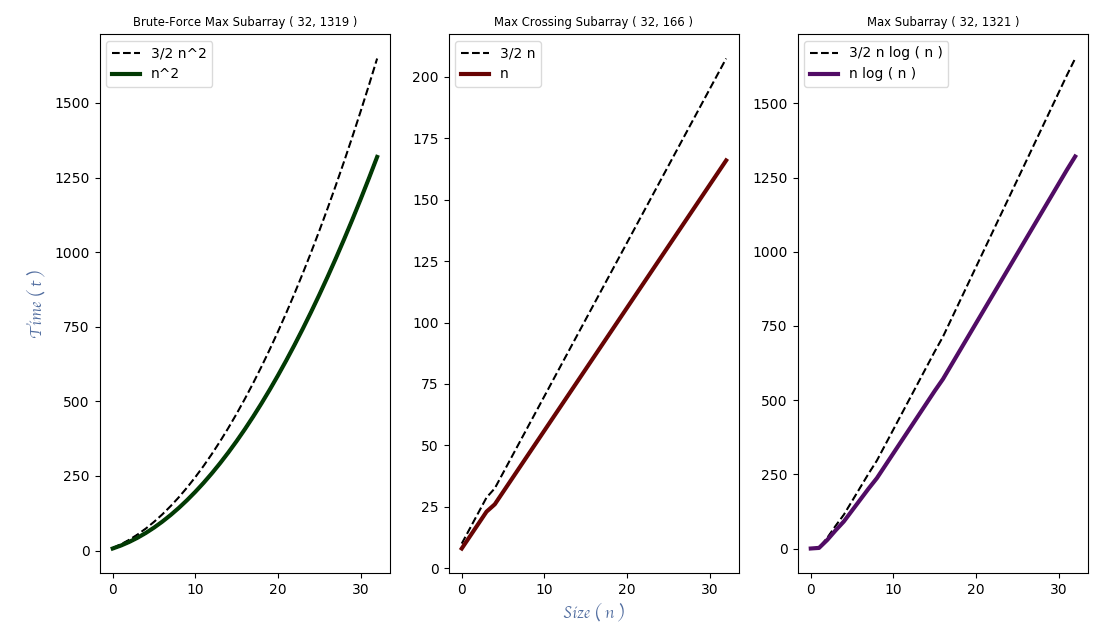
\includegraphics[width = 17cm, height = 10cm]{t2.png}
\centering \linebreak \linebreak Figure 4.1.2: Algorithms running time for an array of size $2^{5}$.
\end{figure} \hfill 

\pagebreak

The following table shows the points of the plots where the first column it's the {\itshape Size} of the array, the second, third and fourth columns describes the computational time of {\itshape Brute-Force}, {\itshape Crossing} and {\itshape Recurrence} Maximum Subarray Algorithms respectively. \hfill \break

\begin{center} 
\begin{tabular}[.5cm]{ c c c c } 
\toprule 
\hspace{10pt} Size ( n ) \hspace{10pt} & \hspace{10pt} Brute-Force Time ( t ) \hspace{10pt} & \hspace{10pt} Crossing Time ( t ) \hspace{10pt} & \hspace{10pt} Recurrence Time ( t ) \\ 
\midrule 
0 & 7 & 8 & 0 \\ 
\cmidrule {1-4} 
1 & 17 & 13 & 2 \\ 
\cmidrule {1-4} 
2 & 29 & 18 & 29 \\ 
\cmidrule {1-4} 
3 & 43 & 23 & 61 \\ 
\cmidrule {1-4} 
4 & 59 & 26 & 91 \\ 
\cmidrule {1-4} 
5 & 77 & 31 & 128 \\ 
\cmidrule {1-4} 
6 & 97 & 36 & 165 \\ 
\cmidrule {1-4} 
7 & 119 & 41 & 202 \\ 
\cmidrule {1-4} 
8 & 143 & 46 & 237 \\ 
\cmidrule {1-4} 
9 & 169 & 51 & 279 \\ 
\cmidrule {1-4} 
10 & 197 & 56 & 321 \\ 
\cmidrule {1-4} 
11 & 227 & 61 & 363 \\ 
\cmidrule {1-4} 
12 & 259 & 66 & 405 \\ 
\cmidrule {1-4} 
13 & 293 & 71 & 447 \\ 
\cmidrule {1-4} 
14 & 329 & 76 & 489 \\ 
\cmidrule {1-4} 
15 & 367 & 81 & 531 \\ 
\cmidrule {1-4} 
16 & 407 & 86 & 571 \\ 
\cmidrule {1-4} 
17 & 449 & 91 & 618 \\ 
\cmidrule {1-4} 
18 & 493 & 96 & 665 \\ 
\cmidrule {1-4} 
19 & 539 & 101 & 712 \\ 
\cmidrule {1-4} 
20 & 587 & 106 & 759 \\ 
\cmidrule {1-4} 
21 & 637 & 111 & 806 \\ 
\cmidrule {1-4} 
22 & 689 & 116 & 853 \\ 
\cmidrule {1-4} 
23 & 743 & 121 & 900 \\ 
\cmidrule {1-4} 
24 & 799 & 126 & 947 \\ 
\cmidrule {1-4} 
25 & 857 & 131 & 994 \\ 
\cmidrule {1-4} 
26 & 917 & 136 & 1041 \\ 
\cmidrule {1-4} 
27 & 979 & 141 & 1088 \\ 
\cmidrule {1-4} 
28 & 1043 & 146 & 1135 \\ 
\cmidrule {1-4} 
29 & 1109 & 151 & 1182 \\ 
\cmidrule {1-4} 
30 & 1177 & 156 & 1229 \\ 
\cmidrule {1-4} 
31 & 1247 & 161 & 1276 \\ 
\cmidrule {1-4} 
32 & 1319 & 166 & 1321 \\ 
\bottomrule 
\linebreak 
\end{tabular} 
\linebreak \linebreak Table 1: Plot points for Figure 4.1.2.
\end{center} \hfill 

\pagebreak


